% LSINF2345 - Languages & Algorithms for distributed applications
% Biker Project
\documentclass[a4paper, 11pt]{article}
\usepackage[utf8]{inputenc}
\usepackage[UKenglish]{babel}
\usepackage{graphicx}				% Use pdf, png, jpg, or eps§ with pdflatex; use eps in DVI mode
\usepackage{xcolor}
\usepackage{listings}
\usepackage{hyperref}
\usepackage{array}
\usepackage{longtable}
\usepackage{multirow}
\usepackage[babel=true]{csquotes}
\usepackage{todonotes}
\usepackage{graphicx}
\usepackage{multicol}
\usepackage{subfig}
\usepackage{tablefootnote}


\usepackage[T1]{fontenc}

\lstset{%
	basicstyle=\ttfamily\footnotesize,
	commentstyle=\color{green!90!black},
	frame=none,
	keywordstyle=\bfseries\color{blue},
	language=python,
	numberstyle=\color{gray},
%	tabsize=2,
}


\hypersetup{%
	colorlinks=true,
	linkcolor=blue,
	urlcolor=blue
}

% Styling commands
\newcommand{\tbf}[1]{\textbf{#1}}
\newcommand{\tit}[1]{\textit{#1}}
\newcommand{\ttt}[1]{\texttt{#1}}

% Semantic commands
\newcommand{\data}[1]{\textit{#1}}
\newcommand{\state}[1]{\textsf{#1}}



\def\blurb{\textsc{Université catholique de Louvain\\
  École polytechnique de Louvain\\
  Pôle d'ingénierie informatique}}
\def\clap#1{\hbox to 0pt{\hss #1\hss}}%
\def\ligne#1{%
  \hbox to \hsize{%
    \vbox{\centering #1}}}%
\def\haut#1#2#3{%
  \hbox to \hsize{%
    \rlap{\vtop{\raggedright #1}}%
    \hss
    \clap{\vbox{\vfill\centering #2\vfill}}%
    \hss
    \llap{\vtop{\raggedleft #3}}}}%
\begin{document}

\begin{titlepage}
\thispagestyle{empty}\vbox to 1\vsize{%
  \vss
  \vbox to 1\vsize{%
    \haut{\raisebox{-2mm}{
\includegraphics[width=2.5cm]{logo_epl.jpg}}}{\blurb}{\raisebox{-5mm}{
\includegraphics[scale=0.20]{ingi_logo.png}}}
    \vfill
    \ligne{\Huge \textbf{\textsc{LSINF2345}}}
     \vspace{5mm}
    \ligne{\huge \textbf{\textsc{Languages \& Algorithms for distributed applications}}}
     \vspace{15mm}
    \ligne{\Large \textbf{\textsc{Biker project}}}
    \vspace{5mm}
    \ligne{\large{\textsc{May 11, 2016}}}
    \vfill
    \vspace{5mm}
    \ligne{%
         \textsc{Professor\\Peter Van Roy}
      }
      \vspace{10mm}
    }%
    \ligne{%
         \textsc{Michael Heraly\\Thibault Gerondal}
      }
      \vspace{5mm}
  \vss
  }
\end{titlepage}



\section*{Introduction}
In this project, we were asked to create a system that simulates a biker race using different solutions for the communication between bikers. However, we had to do it over Riak which is already handling a communication system.

\section{Riak Core}

Riak Core is a distributed systems framework for building distributed, scalable, fault-tolerant applications.
It is based on principles described in the Amazon Dynamo paper ("Dynamo: Amazon’s Highly Available Key-value Store").
However, Riak core is not specially a KV-Store, as Dynamo, but gives us a great support to build such applications. \\

As in Dynamo, Riak core is using a "ring" which is a partitioning scheme that relies on consistent hashing to distribute the load across multiple nodes.
Each node is responsible for regions in the ring.
Each command sent to the system is assigned to a node by hashing the command.
You can also ask to get a preference list of N nodes which will give you a list of hashes distributed on multiple nodes that will execute it.
That is essential in order to have redondancy if a node crash.
As node can join and leave the ring, the riak framework redistribute the partitions between hosts that are alive in the system.
Moreover, when a node leaves the system, only immediate neighbors of this node on the ring are affected and other nodes remain unaffected.
This is important to have a better scalability.\\

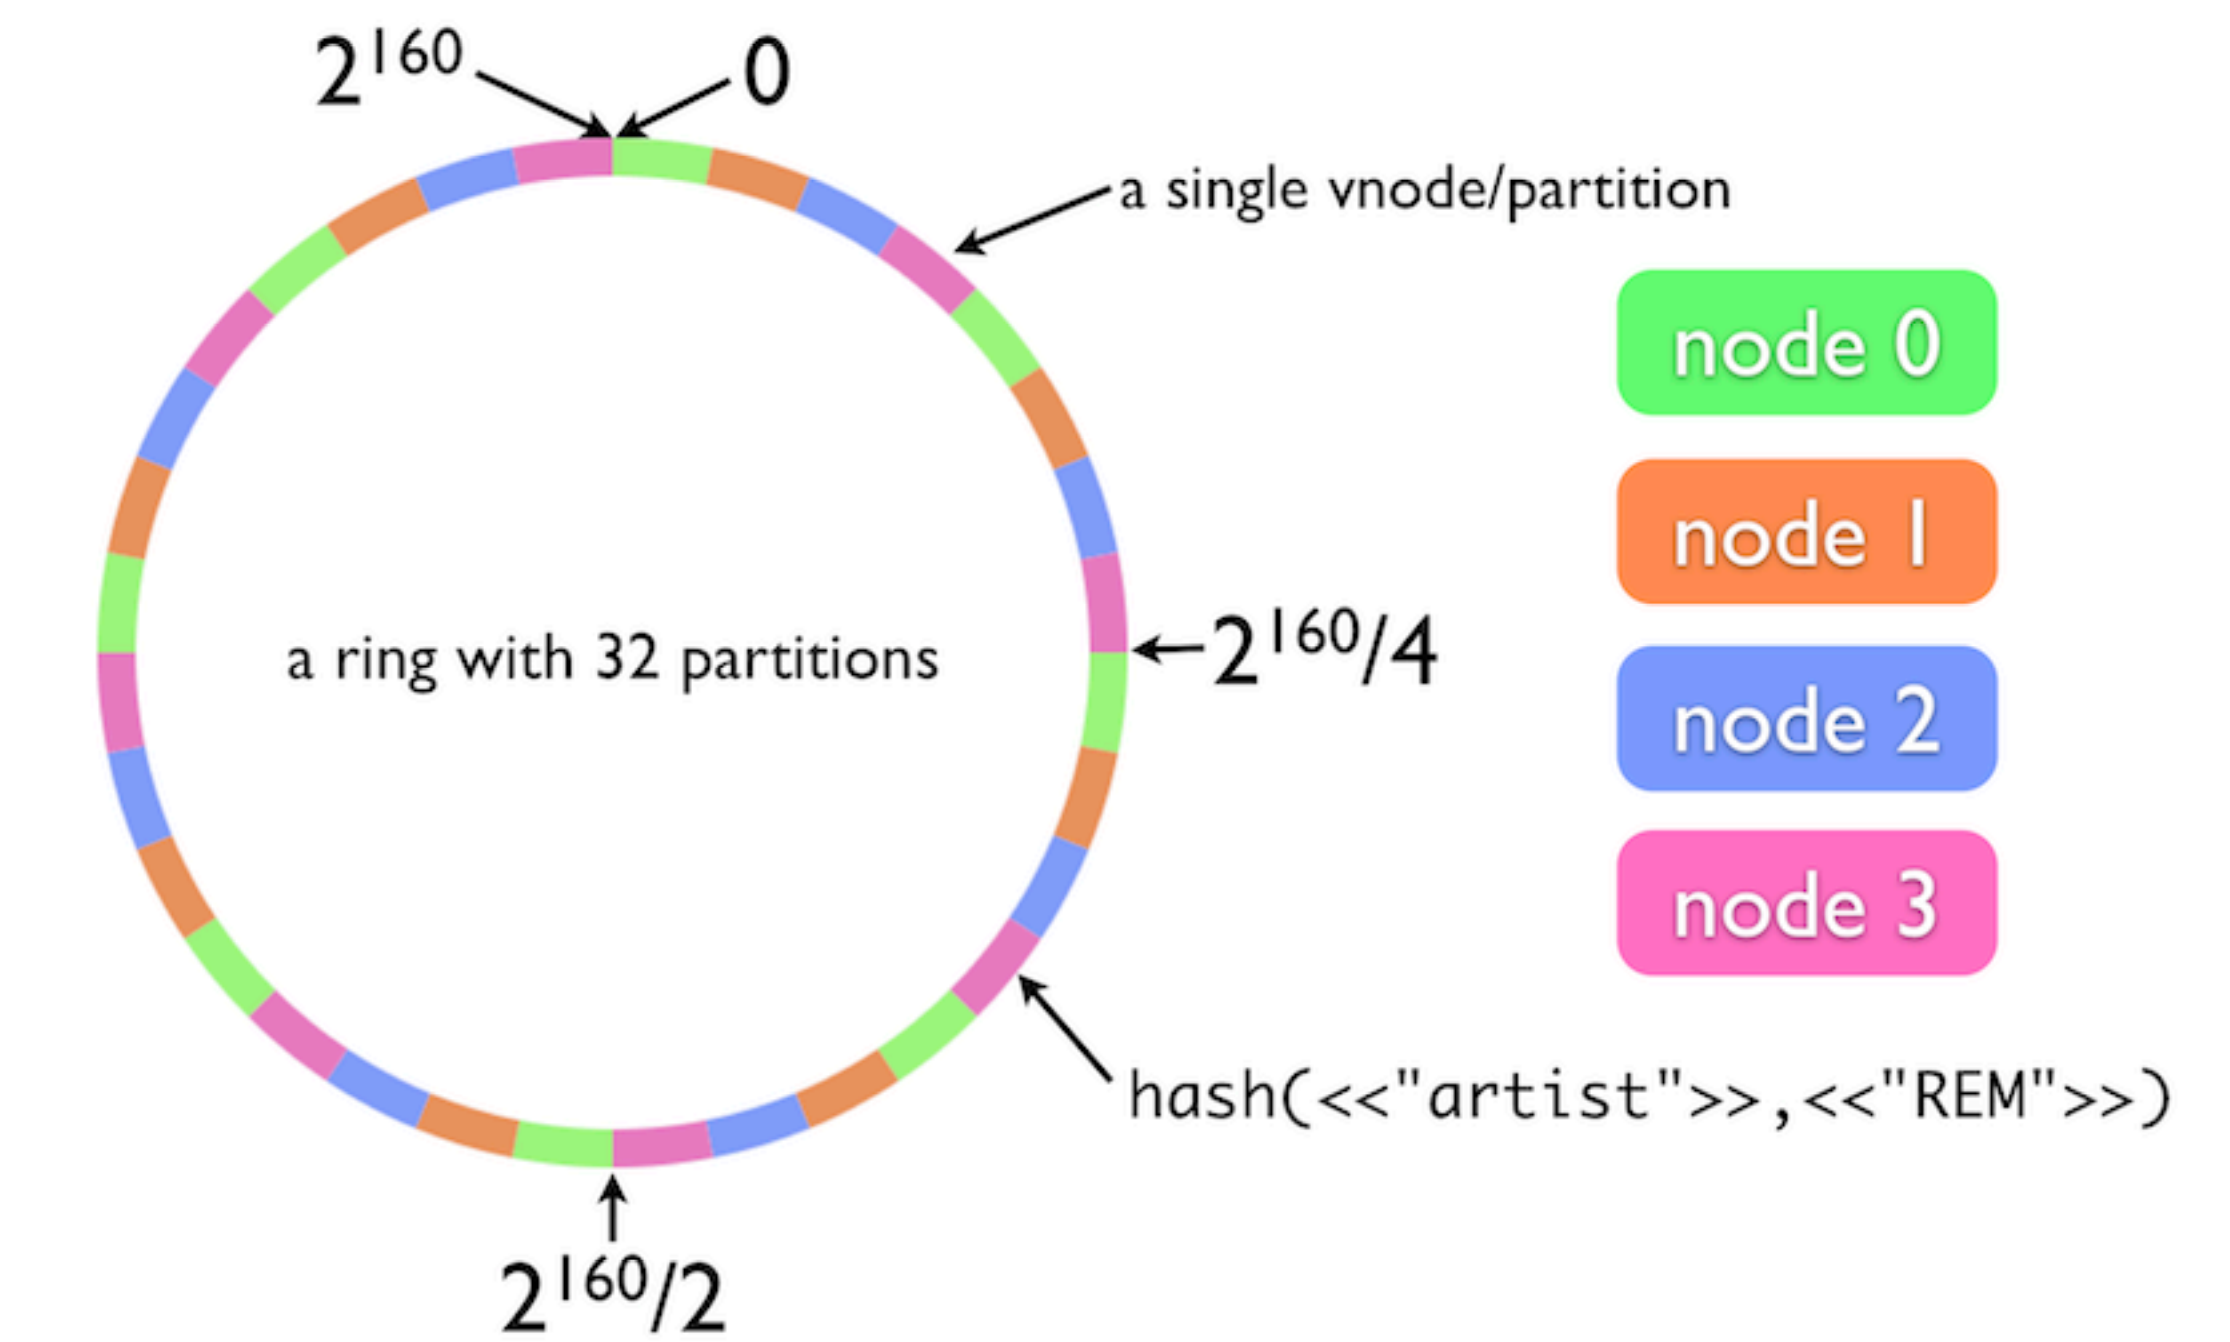
\includegraphics[width=\linewidth]{ring.png}

\newpage
Riak-Core offers a great facility for the management of such distributed infrastructure.
It does not let us choose where our command will be executed as this would break the whole principle of the framework.
Thus, it does not make sense to implement communication algorithms on top of it. \\

However, we did the project as requested over Riak, even if it does not make any sense as any application that wants to use Riak-Core must be studied with the idea of the ring in its core. \\

\section{Biker race}

Each biker is launched on a console of a node in the application.
Every biker keeps track of the race by storing the state of the other bikers within a list.
The state of a biker is represented by a record containing the following keys:
\begin{description}
	\item[id] identifier of the biker,
	\item[position] distance travelled by the biker,
	\item[speed] current speed of the biker,
	\item[energy] remaining energy of the biker,
	\item[behind] id of the biker which is ahead of the biker,
	\item[boost] whether the boost has been used by the biker.
\end{description}

As suggested by the teaching assistant, the communication on this project will be done over a KVstore implemented over Riak which mimics the behavior of Amazon Dynamo.
This means that when we want to "communicate" with another node, we will put a value on this KVstore to make this value available for the others nodes.
As a specific client does not know when the information is available, it will try every 100ms to retrieve the decisions of other nodes.
This causes a lot of communication between the nodes. \\

\subsection{The "behind" command problem}

A biker can decide to follow another biker by going behind him. It thus consumes less energy. However, as every biker have to decide by round their actions, it is possible that two bikers want to follow them each other, or that A want to follow B that want to follow C that himself want to follow A. etc. \\

To solve this problem, we have decided to use a topological ordering to find the order of execution of the algorithm to be sure that the behin command can be executed without breaking anything. Plus, we can easily detect whenever there is a cycle where bikers should circling (following each others). When this happen, every node can notice it and so we ask users to replay the round as it cannot be executed. \\

\subsection{Notes about the asked points of this project}

\subsubsection{The "Best effort broadcast" part}
To produce a strange behavior as described in the "BEB" part of the assignment, we should have a real-time system, in such a way that messages can be sent by nodes at anytime and make a concurrency problem such that node A and node B would be able to have different views of the state of the race.
But here, as the race proceeds by rounds, this cannot be possible as they will wait to receive the decision of every biker (node) of the system.
The fact that a node can be behind, etc. is not a concurrency problem linked to the "beb" and can be handled as described before with a topological ordering.

\subsubsection{The "Total order broadcast" part}
A TOB ensures that messages are received reliably and in the same order by all participants.
Here, we don't need to be sure that messages will be read in the same order as the application described proceeds by rounds.
We just have to wait for all the decisions of every node. \\

If the application was in real-time, we should have to implement a TOB to solve the problem of the BEB described before (divergent views of the state of the race).
To do this, nodes should elect a leader which will decide the order of the messages.

\subsubsection{The "Failing nodes" part}
It can be important to monitor the nodes in a distributed infrastructure to detect the failure of a node.
In this project, Riak handles it for us. \\

If the application was in real-time, we should have to implement such an algorithm in order to know if a node is down as this node could have been the leader.
We can do it with a simple heartbeat algorithm that will just send a "ping" message to other nodes and these will respond with a "pong".
If the leader goes down, thus we would have to elect a new leader, otherwise the race would not be able to continue.

\section{Code}


We implemented our project over an established KVstore on Riak-Core.
To launch our project, launch 3 nodes (for example), join them.
And then, on each attached node, you'll have to launch the command "kvstore:start\_race(X,N)" where X is the id of the biker (1, 2 or 3 for example) an N is the total number of nodes (3 for example).

\end{document}
